\documentclass[11pt]{article}
\usepackage[margin=1in]{geometry}
\usepackage{amsmath,amssymb,booktabs,graphicx,placeins}
\usepackage[font=small,labelfont=bf]{caption}
\usepackage[colorlinks=true,linkcolor=blue,citecolor=blue,urlcolor=blue]{hyperref}
\usepackage{natbib,microtype,xcolor}
\renewcommand{\baselinestretch}{2}
\makeatletter
\g@addto@macro\@floatboxreset{\def\baselinestretch{1}\normalsize}
\makeatother
\renewcommand{\topfraction}{0.95}
\renewcommand{\bottomfraction}{0.85}
\renewcommand{\textfraction}{0.05}
\renewcommand{\floatpagefraction}{0.80}
\setcounter{topnumber}{3}
\setcounter{bottomnumber}{2}
\setcounter{totalnumber}{5}
\setlength{\textfloatsep}{14pt plus 2pt minus 3pt}
\setlength{\floatsep}{10pt plus 2pt minus 2pt}
\setlength{\intextsep}{12pt plus 2pt minus 2pt}
\setlength{\emergencystretch}{2em}
\newcommand{\Tauc}{\mathrm{T\!-\!AUC}_{\Delta}}
\title{State Aggregation in Dynamic Graph Recovery:\\
Separating Structural Ranking from Temporal Discrimination}
\author{Xuansong Chang\\
\small Stony Brook Institute at Anhui University\\
\small Anhui University, 3 Feixi Road, Shushan District,\\
\small Hefei, Anhui 230039, China\\
\small\texttt{alec.xs.chang@gmail.com}}
\date{}
\begin{document}
\begingroup
\renewcommand{\baselinestretch}{1}\selectfont
\maketitle
\endgroup
\begin{abstract}
Post-estimation aggregation of dynamic graph estimates can improve edge
ranking while weakening recovery of when edges are active. We study this
distinction through paired interventions that hold local lagged-edge scores
fixed while varying their temporal emission. Evaluation separates pooled
AUROC, within-edge temporal AUROC and boundary detection, supported by exact
diagnostic identities for static scores and two-state hard aggregation.
Across 100 independent paired simulations, hard aggregation increases pooled
AUROC from $0.727$ to $0.780$ but reduces within-edge temporal AUROC from
$0.707$ to $0.639$ at the shorter-duration configuration. At the longer-duration
configuration, its temporal gain is $0.038$. Schedule, generator and window
comparisons reveal configuration dependence, including changes in switch
coverage. Shrinkage toward edgewise means improves pooled ranking without
changing temporal order. Retaining window-level residuals restores comparisons
lost through hard-output ties, with a measurable rank jump at a near-zero
positive residual weight. Boundary assessments also depend on zero-score
conventions and threshold references. A segmentation-and-refit comparator
improves pooled ranking without an established within-edge temporal gain.
Together, these findings in two-state linear systems motivate separate
evaluation of structural ranking, temporal discrimination and boundary
detection in dynamic graph recovery.

\end{abstract}
\noindent\textbf{Keywords:} Dynamic graph recovery; temporal discrimination;
boundary detection; state aggregation; evaluation; switching autoregression.

\section{Introduction}
\label{sec:intro}
A time-varying graph estimator must recover which relationships exist and when
they are active. An aggregation step can improve the first objective while
weakening the second. This creates a practical ambiguity: a better ranking of
edges may reflect more accurate long-run structure even when the output loses
information about changes. Evaluation must resolve that ambiguity before a
structural improvement can guide interpretation of a dynamic system.

Grouping local connectivity estimates into recurring states is an established
strategy. Sliding-window functional-connectivity studies use representative
states to describe recurrence, reproducibility and task-related variation
\citep{allen2014tracking,abrol2017replicability,chang2026neurocognitive}.
For graph recovery, the corresponding question is how replacing local estimates
by group summaries changes the recovery of individual edges across time.
Shared observations support a controlled comparison: hold the local scores
fixed and vary grouping, score emission and the decision to execute aggregation.

We distinguish three evaluation targets. Pooled AUROC compares positive and
negative edge--window entries, mixing comparisons within and across edges.
Within-edge temporal AUROC compares an edge's active and inactive windows.
Boundary detection evaluates score changes between adjacent windows.
A static occupancy example and finite-score identities connect these targets
to the information that different emission rules preserve.

The distinctions change the empirical assessment of aggregation. Across
100 independent paired simulations at a short-duration configuration, hard
aggregation raises pooled AUROC from $0.727$ to $0.780$ while reducing
within-edge temporal AUROC from $0.707$ to $0.639$. At a longer-duration
configuration, the within-edge gain is positive. Shrinkage toward each edge's
temporal mean also improves pooled ranking while preserving its temporal order,
showing that this structural benefit can arise without state identification.
Residual controls then locate the comparisons lost when hard aggregation
assigns one score to every window in a group.

\paragraph{Contributions.} Three contributions organise the study.
\begin{itemize}
\item An evaluation protocol separates structural ranking, within-edge temporal
discrimination and boundary detection on shared inputs and local scores.
Static, raw, size-matched and oracle controls reveal when an apparent
improvement depends on the evaluation target.
\item Paired simulations identify contrasting temporal effects of hard
aggregation at two duration configurations. Schedule, generator and window
comparisons show how these effects depend on the evaluated configuration;
score-preserving controls identify structural gains that occur without grouping.
\item Diagnostic identities connect hard-emission performance to state-assignment
discrimination and graph contrast, and decompose residual gains into same-group
and cross-group comparisons. Boundary sensitivities and a segmentation/refit
comparison show how score conventions affect the resulting assessment.
\end{itemize}
The experiments use two-state linear switching systems with local Lasso and
OLS scores. This controlled setting links the evaluation analysis to paired
changes in graph recovery while exposing the roles of window resolution,
score emission and gate acceptance.

\section{Related work}
\label{sec:related}
Post-estimation grouping is exemplified by dynamic functional-connectivity
analysis. \citet{allen2014tracking} cluster regularised windowed covariance
matrices into recurring states, using Manhattan distances and cluster-median
maps. \citet{abrol2017replicability} examine replication of state profiles and
temporal summaries, including dwell times and transitions, with hard clustering
and fuzzy meta-states. Task-fMRI work also relates clustered connectivity
states to ongoing events and behaviour \citep{chang2026neurocognitive}.
These are meaningful validation targets for functional association. They differ
from recovery of the temporal support of individual directed lagged edges.

Using simulated networks with known transitions, \citet{shakil2016evaluation}
already evaluate correlation fidelity, state identification and transition
recovery as window parameters and state durations change. Our comparison
isolates the paired gain of aggregating shared local scores over raw windows
on within-edge temporal AUROC. It distinguishes state-level temporal
summaries from within-edge score ordering, using score-preserving and
residual controls to attribute a change in assessment. The distinction is the effect of aggregation on shared local scores,
evaluated separately from state-level summaries and transition detection.

Lagged structure discovery includes stationary Granger-style models
\citep{granger1969investigating,runge2019detecting}. Joint regime and graph
estimators include Regime-PCMCI, CASTOR and SPACETIME
\citep{saggioro2020regime,rahmani2025castor,mameche2025spacetime}.
Jointly fitting state assignments and graph models changes the local estimates
as well as their grouping. Aggregating fixed scores is a separate intervention.
Penalised changepoint optimisation \citep{killick2012optimal} and VAR break
models \citep{bai1998estimating} motivate the segmentation comparisons in Supplement Section~S6.

Multidimensional evaluation can expose differences that a single structural
score conceals. \citet{velev2026evaluation} evaluate causal discovery from
observational i.i.d.\ data through structural recovery and the suitability of
estimated graphs for causal inference under varying assumptions. Here the
evaluation object is a time-varying graph: rankings across edges and temporal
discrimination within changing edges need separate accounting. The classical
bipartite-ranking principle \citep{clemencon2008ranking} underlies our static
occupancy ceiling; its role here is a task-specific diagnostic.

Evaluation choices also alter comparisons in dynamic link prediction
\citep{poursafaei2022towards}, where simple memory baselines and the choice of
negative examples matter. That task observes a graph and predicts future links.
We instead infer latent lagged support from multivariate series and ask what
grouping windows preserves. Constant-score controls and within-edge temporal AUROC
make this difference assessable.

\section{Problem setup and controlled aggregation framework}
\label{sec:framework}
Let $X_{1:T}\in\mathbb R^{T\times N}$ follow an unobserved state sequence $z_t$.
The binary tensor $A_{k,\ell,i,j}$ marks the lag-$\ell$ support from source $i$
to target $j$ in state $k$. Regression includes self- and cross-lags, but edge
evaluation and clustering exclude self-lag scores. Union evaluation uses
$A_{\cup,\ell,i,j}=\mathbf1\{\exists k:A_{k,\ell,i,j}=1\}$; regime evaluation
matches state identities before scoring; time-indexed evaluation compares each
emitted graph with the true state at its window centre. AUROC, AUPRC and
precision inherit the meaning of the chosen target and indexing.

\subsection{A shared-score aggregation experiment}
\label{sec:method}
We investigate post-estimation state aggregation using a controlled window-based
framework. Local lagged-edge scores are held fixed while grouping, score
emission and the acceptance rule are varied to isolate their effects on graph
recovery. Window length $h$ and stride $s$ give
$M=1+\lfloor(T-h)/s\rfloor$ windows. Each window is standardised per variable;
one Lasso per target is fitted to standardised lagged inputs with
$\alpha=0.005$. Absolute coefficients form scores $S_{w,e}$. Self-lags enter
regression but are excluded from the evaluated edges and clustering features.
Non-self scores are standardised across windows and clustered into a supplied
$K=2$ groups by K-means. The auxiliary OLS scorer uses the same windows,
preprocessing and evaluation. Supplement Section~S2 gives the fitting
procedures; Supplement Section~S4 reports numerical-failure rules and coverage.

For candidate labels $\widehat z_w$, hard aggregation emits the mean score of
each window's group. We distinguish three execution rules. \emph{Forced hard
aggregation} always emits that candidate. \emph{Gated hard aggregation with
static fallback} emits it when a fixed inertia/coherence gate accepts and
otherwise emits the same window-maximum graph at every window.
\emph{Gated hard aggregation with raw fallback} uses the same acceptance
decision and emits the raw window scores on rejection. The gate evaluates
relative inertia improvement, adjacency agreement adjusted for group
proportions, and minimum group size; its full definition is in Supplement
Section~S2. These rules separate candidate quality from the effects of
acceptance and rejection output.

Raw windows emit $S_w$ directly. Static mean emits one temporal-mean graph.
Oracle-label aggregation averages by the true window-centre state without
refitting. In Study A and the earlier selected seven-window comparison at $D=600$,
size-matched random grouping enumerates every unlabelled bipartition with the
candidate's group sizes and averages its metrics within each simulation
repeat. These controls share observations and local scores;
the oracle additionally supplies true state assignments.

\subsection{Generators and paired interventions}
\label{sec:generator}
The simulations use $N=8$ variables, maximum lag $L=3$ and independent
Gaussian innovations with standard deviation $0.10$. Studies A and B use
an asymmetric support construction. State A has non-self support probability
$0.18$ and no self-lags. State B retains each A edge with probability $0.5$
and can add edges, including self-lags, outside A's support; its non-self
marginal probability is $0.1638$ before empty-support safeguards. Coefficients
are redrawn between states, including on shared support. These properties
are fixed throughout A and B. Study C jointly changes support symmetry,
self-lags, shared coefficients and the stabilisation rule to assess a separate
generator construction. Supplement Section~S2 specifies the A/B mechanism;
Section~S4.2 specifies the C mechanism and its window configurations.

Each independent repeat redraws the graph mechanism, initial history and
innovations. Conditions within a repeat share all three, making their
differences paired. After 100 burn-in samples, records alternate between
two states under fixed-duration, random-phase or irregular-duration schedules.
At fixed series length, changing duration also changes the number and coverage
of observed transitions. Window length, stride, window count and realised
switch counts are therefore reported alongside duration.
Post-scaling companion radii are $0.381$--$0.676$ in A and
$0.404$--$0.627$ in B, and all 500 observed A/B trajectories are finite.
Supplement Section~S8 reports the associated trajectory diagnostics.

OpenAI Codex (OpenAI) assisted implementation, regression testing, experiment
orchestration and plotting code. Figures are generated by reproducible Python
scripts from the numerical outputs and the specified finite example. The
reproducibility archive supplies these scripts and their inputs; the end-matter
declaration describes the broader use of AI and author responsibility.

\section{Evaluation and mechanism analysis}
\label{sec:evaluation}
\subsection{Pooled ranking and within-edge temporal discrimination}
\label{sec:static-occupancy}
For edge occupancy $\pi_e=M^{-1}\sum_{w=1}^{M} A_{w,e}$ and constant scores $s_e$,
writing $H(u)=\mathbf1(u>0)+\tfrac12\mathbf1(u=0)$, pooled AUROC is
\begin{equation}
\mathrm{AUC}_{\rm static}
=\frac{\sum_{e,f}\pi_e(1-\pi_f)H(s_e-s_f)}
{P Q},\qquad P=\sum_e\pi_e,\quad Q=\sum_e(1-\pi_e).
\label{eq:auc-static}
\end{equation}
It depends on frequencies rather than activation times. Sorting edges by
$\pi_e$ is optimal among constant scores: an adjacent exchange changes the
numerator by the difference in occupancies. Classical optimal ranking thus gives
\begin{equation}
\mathrm{AUC}_{\rm static}^{*}
=\tfrac12+\frac{\sum_{e,f}|\pi_e-\pi_f|}{4P Q}.
\label{eq:static-ceiling}
\end{equation}
This ceiling characterises the ranking attainable from occupancy alone.

For general time-indexed scores, the positive--negative comparison pairs split
exactly into same-edge and cross-edge parts:
\begin{equation}
\mathrm{AUC}_{\rm pooled}=\omega\mathrm{AUC}_{\rm same}
+(1-\omega)\mathrm{AUC}_{\rm cross},\qquad
\omega=\frac{\sum_e n_e^+n_e^-}{(\sum_e n_e^+)(\sum_e n_e^-)}.
\label{eq:pooled-split}
\end{equation}
Here $n_e^+=\sum_{w=1}^{M} A_{w,e}$ and $n_e^-=M-n_e^+$ count the
positive and negative window labels of edge $e$ on the same evaluation grid.
Cross-edge comparisons can also depend on time. Equation~\eqref{eq:pooled-split}
therefore identifies the mixture of comparisons in pooled AUROC, with its
same-edge weight determined by the evaluation labels.

Let $\mathcal E_\Delta$ contain non-self lagged edges whose binary label changes
in the evaluation windows. Within-edge temporal AUROC on changing edges is
\begin{equation}
\Tauc=|\mathcal E_\Delta|^{-1}
\sum_{e\in\mathcal E_\Delta}\mathrm{AUROC}
\bigl((A_{w,e})_w,(\widehat S_{w,e})_w\bigr).
\label{eq:temporal-target}
\end{equation}
An edge without both positive and negative evaluation labels is not scored;
undefined targets remain missing. Constant emission scores $0.5$ whenever
this target is defined. Figure~\ref{fig:targets} illustrates why high pooled
ranking need not imply within-edge temporal discrimination.
Equation~\eqref{eq:temporal-target} measures the ordering of an edge's active
and inactive windows. It does not measure distance to a switch boundary,
and it excludes edges whose support is constant. Permuting scores within the
active windows, or within the inactive windows, leaves it unchanged while
potentially changing the locations of thresholded errors. We therefore also evaluate boundary detection and variation on stable edges.

\paragraph{Boundary-slot detection.}
A slot is the interval between consecutive window centres. It is positive for
an edge if its true support changes at least once in that interval, and the
predicted change strength is the absolute difference between consecutive
emitted scores. This target evaluates change detection at stride resolution.
We report boundary-detection AP and F1, together with false changes on stable
edges. Standard AP includes the zero-score group; positive-change AP treats
zero strength as abstention. Supplement Section~S1 summarises slot targets;
Section~S5 defines threshold references and AP conventions, compared here
in Section~\ref{sec:localisation-results}.

\begin{figure}[!htbp]
\centering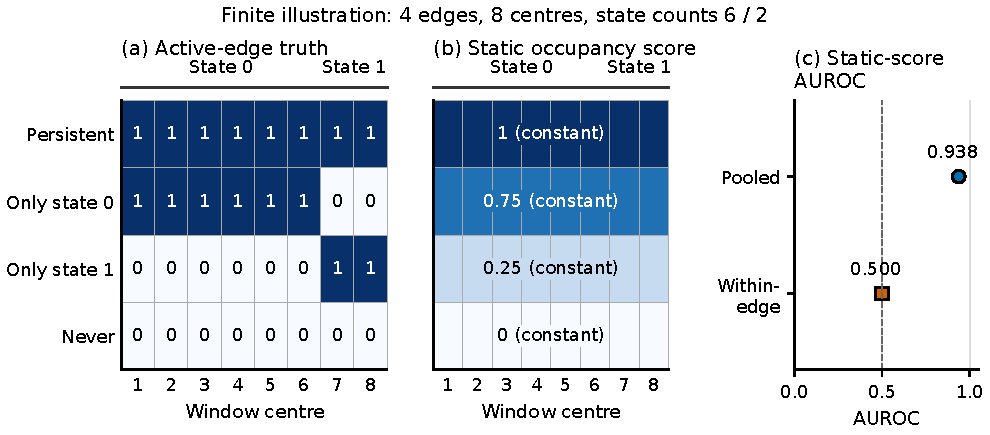
\includegraphics[width=\linewidth]{results/information_sciences/narrative_assets/fig_target_example.pdf}
\caption{A deterministic evaluation example, not an empirical estimate.
Time-indexed truth is compared with constant occupancy scores. The static
predictor can rank frequent edges accurately while having within-edge
temporal AUROC $0.5$. The underlying truth and scores accompany the figure.}
\label{fig:targets}
\end{figure}

\subsection{Two-state hard emission and relative gain}
\label{sec:state-factor}
With two true states and two fixed predicted maps, align state numbering once.
Define state-assignment discrimination
$J=\Pr(\widehat z=1\mid z=1)-\Pr(\widehat z=1\mid z=0)$ and, for changing edges,
\begin{equation}
C_{\rm edge}=|\mathcal E_\Delta|^{-1}
\sum_{e\in\mathcal E_\Delta}
\operatorname{sign}\!\left[(A_{1,e}-A_{0,e})(G_{1,e}-G_{0,e})\right].
\end{equation}
The two possible emitted scores per edge make its AUROC depend only on
state-assignment discrimination and the direction of the map difference, yielding
\begin{equation}
\Tauc=\tfrac12+\tfrac12 J C_{\rm edge}.
\label{eq:state-factor}
\end{equation}
The identity is invariant to exchanging predicted state names. Across repeats,
the mean of products is required; marginal means must not be multiplied.
For the same repeat set, with $T$ denoting Eq.~\eqref{eq:temporal-target},
\begin{equation}
\overline\Delta_{\rm temporal}
=\overline T_{\rm hard}-\overline T_{\rm raw}
=\tfrac12\left[\overline{JC_{\rm edge}}
-(2\overline T_{\rm raw}-1)\right].
\label{eq:temporal-gain-factor}
\end{equation}
The identity makes relative gain explicit: the mean grouping--contrast product
must exceed the raw score's temporal-ranking reference for a positive mean
hard-minus-raw difference. Both factors use ground-truth states and changing
edges, so this is a retrospective diagnostic of the evaluated configuration.
The occupancy and comparison identities apply to finite arrays independently
of the local scorer; the factorisation requires two true states and two
emitted maps. Supplement Section~S3 gives the derivations and auxiliary
window-mixing and risk analyses.

The specified gate has a separate geometric property. With seven windows,
optimal two-group inertia improvement is at least $1/6$, exceeding its $0.12$
acceptance threshold even without state structure. The bound concerns the
optimal partition; actual K-means fits and gate outcomes are measured
separately. This motivates reporting forced candidates and both fallback
rules alongside acceptance rates (Supplement Section~S3).

\subsection{Score-preserving controls and the fallback decision}
\label{sec:score-controls}
For each edge, let $\overline S_e=M^{-1}\sum_w S_{w,e}$. Global shrinkage
\begin{equation}
S^{\rm shrink}_{w,e}=\lambda S_{w,e}+(1-\lambda)\overline S_e,
\qquad 0<\lambda\leq1,
\label{eq:score-shrink}
\end{equation}
preserves every within-edge comparison, including ties, in exact arithmetic:
$S^{\rm shrink}_{u,e}-S^{\rm shrink}_{v,e}
=\lambda(S_{u,e}-S_{v,e})$. Hence it preserves
Eq.~\eqref{eq:temporal-target} for any graph generator and any local scorer.
Across different edges, the edge-specific offsets can change pooled rankings.
This gives a non-clustering control for structural improvement with temporal
order preserved: any pooled gain under this intervention arises through
changed cross-edge comparisons.

We also retain window residuals around the candidate hard emission $H_{w,e}$:
\begin{equation}
S^{\rm residual}_{w,e}=H_{w,e}+\lambda(S_{w,e}-H_{w,e}).
\label{eq:score-residual}
\end{equation}
This interpolates between hard ($\lambda=0$) and raw ($\lambda=1$).
Its edgewise ordering across candidate groups need not equal raw ordering.
Within a common candidate group, $H_{u,e}=H_{v,e}$ and the residual score
difference is $\lambda(S_{u,e}-S_{v,e})$. Thus every positive weight restores
that group's raw ordering, whereas hard emission ties those comparisons.
AUROC can jump at zero residual weight; it need not improve smoothly with
the retained amplitude. We account for same-group and cross-group pair
contributions separately, including a diagnostic near-zero weight.
We report all fixed values $\lambda\in\{0.25,0.5,0.75,1\}$ for both controls,
alongside the hard endpoint, without choosing a value using the evaluation
truth. The implementation checks actual finite-precision order and tie changes.

Let $I$ indicate the fixed gate's acceptance and $T$ the within-edge
temporal AUROC of one repeat. Emitting raw on rejection gives
\begin{equation}
\Delta_{\rm raw\,fallback}=I(T_{\rm hard}-T_{\rm raw}),\qquad
\Delta_{\rm static\,fallback}=I(T_{\rm hard}-T_{\rm raw})
 +(1-I)(\tfrac12-T_{\rm raw}).
\label{eq:fallback-decomposition}
\end{equation}
Thus the difference between the two fallback rules isolates information lost
by constant emission on rejection. The mean raw-fallback gain is the acceptance
rate times the accepted subset's own mean hard-minus-raw gain. This separates candidate selection from information discarded by the
rejection output.

\section{Controlled empirical study}
\label{sec:empirical}
\subsection{Experimental design and statistical inference}
Table~\ref{tab:protocol} summarises the three simulation studies. Study A
compares two duration configurations in 100 independent paired repeats.
Pilot experiments informed the selected configurations; the primary contrasts
and multiplicity adjustments were specified before the corresponding
confirmatory simulations. Its primary family contains four Lasso contrasts:
gated hard minus raw at each duration; their within-repeat difference
$\Gamma=\mathbb E[\Delta(600)-\Delta(300)]$; and hard minus size-matched
random grouping at $D=600$. Two-sided repeat-level t tests use Holm correction
across these four contrasts. OLS and forced-hard comparisons are prespecified
auxiliary analyses.

Study B uses 50 different independent repeats to compare two mean durations
under fixed, random-phase and irregular schedules. Its six forced-minus-raw
comparisons form a secondary Holm6 family, and its three paired duration
differences form a separate secondary Holm3 family. Study C is a separately
specified robustness study with 30 further independent repeats, two durations
and five window/stride settings. Studies A--C are reported separately; they
were not externally preregistered. Supplement Section~S4 gives their complete
designs, seed ranges, contrasts and numerical coverage.

Additional score-emission controls use the fitted predictions from these
studies. The AP, threshold and near-zero-residual sensitivity settings were
chosen after A--C results were available, and the fixed segmentation/refit
comparison uses existing Study C cases. These analyses are exploratory and
remain outside the primary confirmatory family. All intervals are pointwise
$95\%$ percentile bootstrap intervals based on 10,000 repeat resamples;
paired differences are computed within repeat before summarisation. Repeats,
rather than windows, edges or random partitions, are the statistical units.
Fit failures and undefined targets are reported with their denominators.

\begin{table}[!htbp]\centering
\caption{Simulation designs. Within a repeat, conditions share graph coefficients,
support, initial history and innovations. Window length/stride are denoted $h/s$;
Study C's five settings assess window resolution under a separate generator.
Primary, secondary and exploratory analyses use the distinct inference rules
described in the text.}
\label{tab:protocol}
\resizebox{\linewidth}{!}{\begin{tabular}{llrll}
\toprule
Study: repeats / seeds & Paired design & $T$ & Window grid: $h/s$; $M$ & Statistical role \\
\midrule
\shortstack[l]{A: 100 independent repeats\\50000--50099} & \shortstack[l]{Fixed phase; $D=300,600$\\Two cells per repeat} & 1200 & $300/150$; $7$ & \shortstack[l]{Confirmation: gated Lasso Holm4\\Forced and OLS auxiliary} \\
\shortstack[l]{B: 50 independent repeats\\60000--60049} & \shortstack[l]{Fixed/random/irregular\\$\bar D=300,600$; six cells} & 3600 & $300/150$; $23$ & \shortstack[l]{Secondary robustness\\Forced--raw Holm6; duration Holm3} \\
\shortstack[l]{C: 30 independent repeats\\70000--70029} & \shortstack[l]{Symmetric generator\\$D=300,600$; ten cells} & 3600 & \shortstack[l]{$200/100$; $35$\\$300/150$; $23$\\$400/200$; $17$\\$300/75$; $45$\\$300/300$; $12$} & \shortstack[l]{Separate robustness study\\Pointwise 95\% intervals\\No confirmatory family} \\
\bottomrule
\end{tabular}
}
\end{table}

\subsection{Structural ranking gains versus temporal discrimination}
Hard aggregation improves pooled ranking while having opposite temporal
effects at the two duration configurations (Table~\ref{tab:study-a-main}(a)).
At $D=300$, pooled AUROC rises from $0.727$ to $0.780$, while within-edge
temporal AUROC falls from $0.707$ to $0.639$. The paired temporal difference
is $-0.069$ $[-0.090,-0.048]$, compared with $+0.038$ $[0.023,0.053]$
at $D=600$. Their direct paired difference is $\Gamma=+0.107$
$[0.079,0.134]$. Hard aggregation also exceeds size-matched random grouping
by $+0.226$ $[0.210,0.243]$ at $D=600$. All four primary comparisons pass
Holm4 correction; the largest adjusted p value is $2.93\times10^{-6}$.

All 400 Lasso/OLS fits succeed and all temporal targets are evaluable. The
gate accepts all $100/100$ fits at both durations, so gated and forced hard
outputs coincide here. The observed records contain four versus two switches,
and the seven window centres contain three versus one switches, at
$D=300$ versus $600$. Thus Figure~\ref{fig:confirmation} compares two
complete duration/coverage configurations.

The prespecified OLS check yields the same contrast: hard-minus-raw is
$-0.071$ $[-0.092,-0.051]$ at $D=300$ and $+0.032$ $[0.017,0.046]$
at $D=600$, with paired difference $+0.103$ $[0.076,0.129]$.
Supplement Section~S4 reports all contrasts, scores and fit diagnostics.

\begin{table}[!htbp]\centering
\caption{Study A: mean pooled and within-edge temporal AUROC on the same
independent repeats. All methods share local Lasso scores within each fit.
Intervals and the four primary comparisons are shown in Figure~\ref{fig:confirmation};
coverage and failure counts are reported in Supplement Section~S4.
Paired differences are computed before rounding: the displayed marginal means
$0.639$ and $0.707$ do not determine the displayed difference $-0.069$.}
\label{tab:main-results}
\resizebox{\linewidth}{!}{\begin{tabular}{lrrrr}
\toprule
 & \multicolumn{2}{c}{$D=300$} & \multicolumn{2}{c}{$D=600$} \\
\cmidrule(lr){2-3}\cmidrule(lr){4-5}
Method & Pooled AUROC & Within-edge AUROC & Pooled AUROC & Within-edge AUROC \\
\midrule
Raw windows & 0.727 & 0.707 & 0.772 & 0.767 \\
Static mean & 0.806 & 0.500 & 0.841 & 0.500 \\
Gated hard & 0.780 & 0.639 & 0.839 & 0.805 \\
Forced hard & 0.780 & 0.639 & 0.839 & 0.805 \\
Matched random & 0.779 & 0.559 & 0.817 & 0.579 \\
Oracle labels & 0.803 & 0.797 & 0.846 & 0.848 \\
\bottomrule
\end{tabular}
}
\end{table}
\begin{figure}[!htbp]\centering
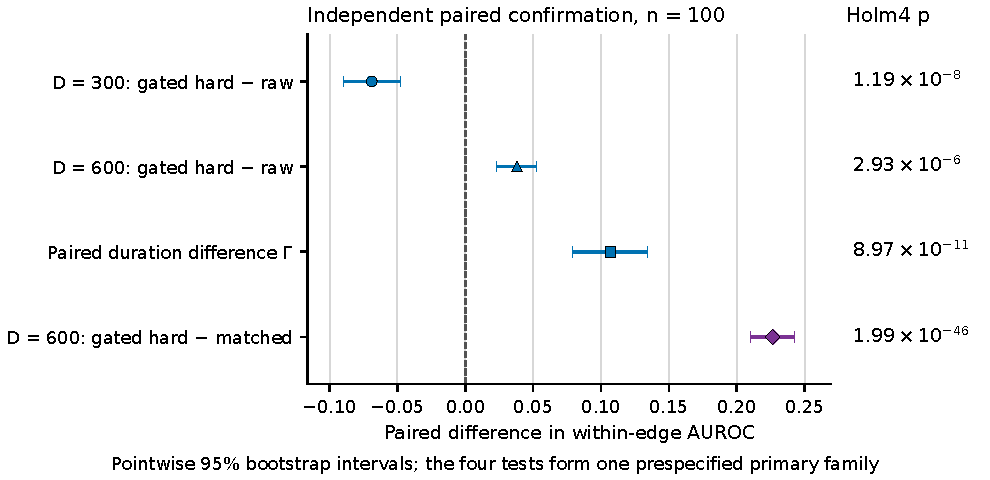
\includegraphics[width=\linewidth]{results/information_sciences/narrative_assets/fig_confirmation.pdf}
\caption{Study A: paired repeat differences and the four-comparison
primary family. Intervals are pointwise $95\%$ bootstrap intervals; p values
are two-sided t tests with Holm4 adjustment. Duration differences are paired
within the same mechanism/noise repeat.}
\label{fig:confirmation}
\end{figure}

\subsection{Sensitivity to switching schedules and gate acceptance}
Positive candidate effects at $D=600$ persist across the three switching
schedules (Figure~\ref{fig:schedule}). Forced hard-minus-raw within-edge
temporal AUROC is $+0.072$ $[0.055,0.089]$ for fixed phase, $+0.072$
$[0.050,0.094]$ for random phase and $+0.070$ $[0.047,0.091]$ for
irregular runs; all three pass secondary Holm6 correction. At $D=300$,
the estimates are $-0.025$, $+0.003$ and $-0.019$, with intervals crossing
zero. The paired duration differences are $+0.097$, $+0.070$ and $+0.089$,
all passing the separate secondary Holm3 family. All six cells have 50
successful, evaluable repeats (300 condition fits in total). The fixed-phase records contain eleven/five
window-centre switches, extending the three/one-switch contrast of Study A.

Gate acceptance changes the effect of executing this candidate. Acceptance
is $2/50$, $0/50$, $3/50$ at $D=300$ and $6/50$, $6/50$, $7/50$
at $D=600$ for fixed, random and irregular schedules. Gated hard aggregation
with static fallback has negative gains throughout, from $-0.214$ to
$-0.198$ (Figure~\ref{fig:gate}). Section~\ref{sec:control-results} examines
how much of that loss comes from the rejection output.

The factor diagnostics in Table~\ref{tab:factors} account for the stronger
forced candidates at the longer duration. Mean per-repeat $JC_{\rm edge}$
is approximately $0.666$, $0.656$ and $0.659$ at $D=600$, compared with
$0.358$, $0.400$ and $0.363$ at $D=300$. State-assignment discrimination
and graph-contrast concordance change together in these comparisons.

\begin{figure}[!htbp]\centering
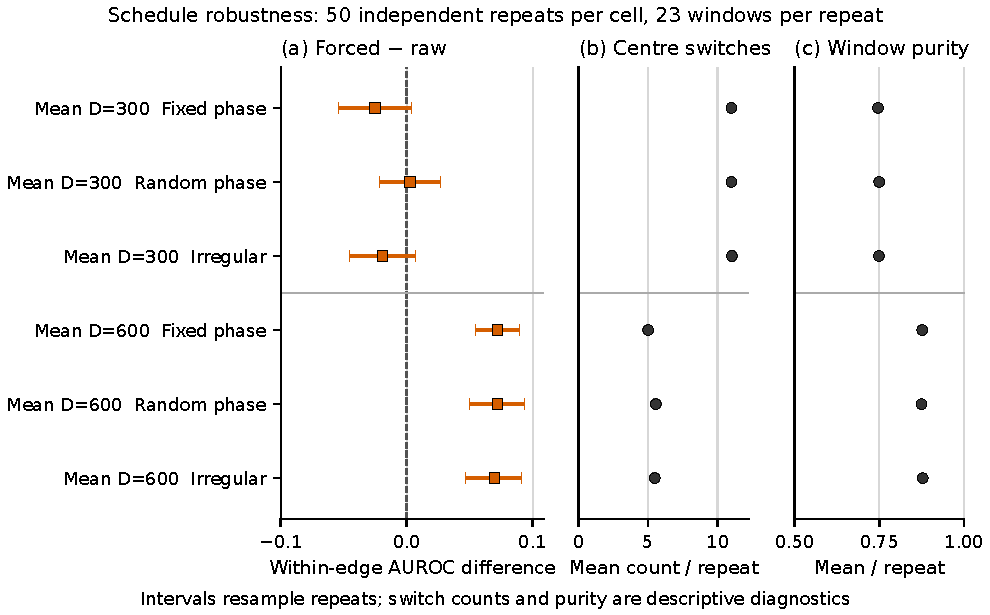
\includegraphics[width=\linewidth]{results/information_sciences/narrative_assets/fig_schedule.pdf}
\caption{Study B: forced aggregation gains, realised window-centre switch
counts and mean window purity for all six planned cells. Points/intervals use
independent simulation repeats.
The schedule comparisons are secondary robustness analyses.}
\label{fig:schedule}
\end{figure}
\begin{table}[!htbp]\centering
\caption{Candidate-hard factor diagnostics. Every row uses all evaluable forced
candidates, including gate rejections. Per-repeat products are averaged across repeats;
raw reference is $2\overline T_{\rm raw}-1$. Differences among jointly estimated
factors are descriptive.}
\label{tab:factors}
\resizebox{\linewidth}{!}{\begin{tabular}{lrrrrrrr}
\toprule
Study/cell & $D$ or $\bar D$ & $n$ & $\overline J$ & $\overline C_{\rm edge}$ & $\overline{JC_{\rm edge}}$ & $2\overline T_{\rm raw}-1$ & Forced $\Delta$ \\
\midrule
A: Fixed phase & 300 & 100 & 0.550 & 0.406 & 0.277 & 0.415 & -0.069 \\
A: Fixed phase & 600 & 100 & 0.888 & 0.677 & 0.610 & 0.534 & +0.038 \\
B: Fixed phase & 300 & 50 & 0.525 & 0.592 & 0.358 & 0.408 & -0.025 \\
B: Random phase & 300 & 50 & 0.545 & 0.687 & 0.400 & 0.395 & +0.003 \\
B: Irregular & 300 & 50 & 0.510 & 0.651 & 0.363 & 0.402 & -0.019 \\
B: Fixed phase & 600 & 50 & 0.817 & 0.812 & 0.666 & 0.521 & +0.072 \\
B: Random phase & 600 & 50 & 0.807 & 0.807 & 0.656 & 0.511 & +0.072 \\
B: Irregular & 600 & 50 & 0.786 & 0.828 & 0.659 & 0.520 & +0.070 \\
\bottomrule
\end{tabular}
}
\end{table}
\begin{figure}[!htbp]\centering
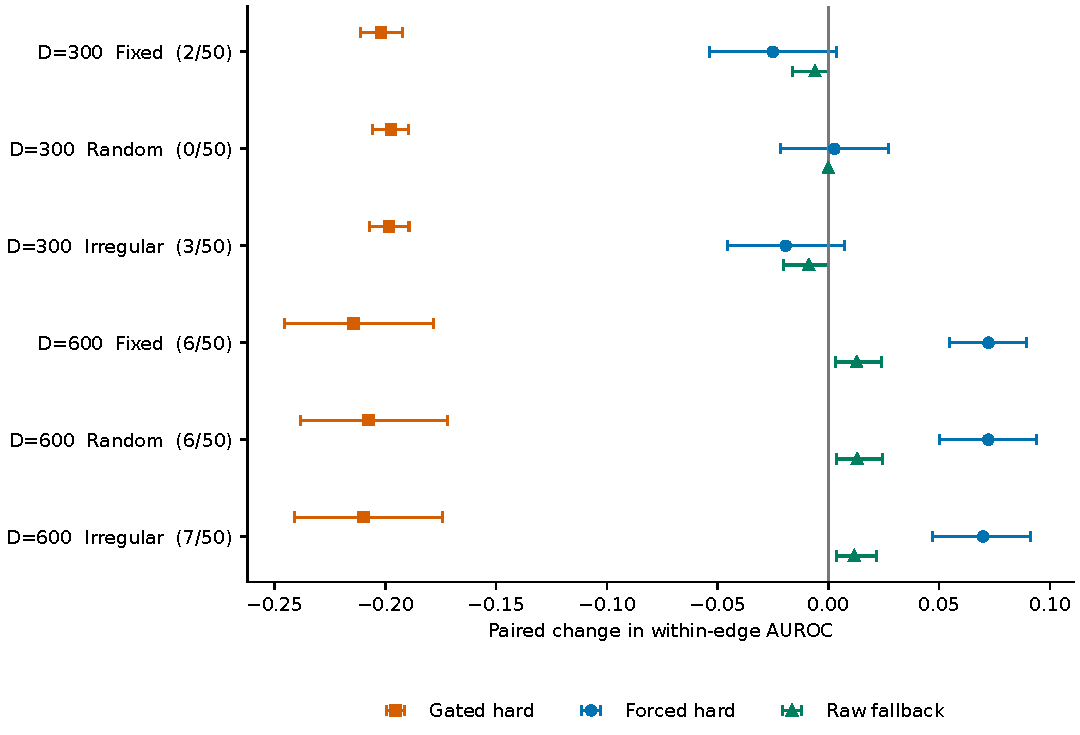
\includegraphics[width=\linewidth]{results/information_sciences/narrative_assets/fig_fallback.pdf}
\caption{Study B with the gate held fixed: gated hard with static fallback, forced
hard emission and raw fallback. Parentheses give accepted/fitted counts.
Intervals are pointwise paired-repeat $95\%$ bootstrap intervals; repeated
hard-aggregation contrasts reuse the Study B summaries (Supplement Section~S5).
Raw fallback
emits the raw windows on rejection, separating gate selection from
information discarded by the rejection output.}
\label{fig:gate}
\end{figure}

\subsection{Disentangling cross-edge gains and within-edge information loss}
\label{sec:control-results}
Pooled ranking gains also arise without grouping (Table~\ref{tab:score-controls}).
In Study A, shrinkage at $\lambda=0.25$ raises pooled AUROC to $0.804$
at $D=300$ and $0.843$ at $D=600$, while preserving the respective raw
within-edge temporal AUROCs $0.707$ and $0.767$. Weights $0.5$ and
$0.75$ also improve pooled ranking. Every positive shrinkage weight preserves
within-edge comparisons, including ties, across the A--C predictions.
Equation~\eqref{eq:score-shrink} attributes these gains to cross-edge reordering.

Window residuals improve the hard-emission comparison. At $D=300$, residual
weights $0.25$, $0.5$ and $0.75$ yield temporal gains over raw of $+0.010$
$[0.001,0.020]$, $+0.009$ $[0.003,0.015]$ and $+0.006$
$[0.003,0.008]$, respectively, compared with hard emission's $-0.069$.
At $D=600$, weight $0.25$ yields $+0.057$ $[0.050,0.064]$, compared
with hard's $+0.038$. These additional analyses report all fixed weights
with pointwise intervals and remain outside the primary confirmatory family.

Changing the rejection output explains much of the gated loss in Study B.
At $D=600$, gains with raw fallback are $+0.013$ $[0.003,0.024]$,
$+0.013$ $[0.004,0.024]$ and $+0.012$ $[0.003,0.022]$ for the
three schedules, compared with static-fallback gains near $-0.21$.
Both rules accept exactly the same candidates. At $D=300$, the corresponding
raw-fallback means are $-0.006$, $0$ and $-0.009$.
Equation~\eqref{eq:fallback-decomposition} separates losses on rejected
repeats from the quality of the accepted candidates.

The pair decomposition locates a rank jump at the hard endpoint. At the
diagnostic weight $10^{-8}$, Study A's Lasso within-edge temporal AUROC
rises from $0.639$ to $0.707$ at $D=300$ and from $0.805$ to $0.830$
at $D=600$. The increases $0.068$ and $0.025$ arise entirely from resolving
same-group positive--negative ties; cross-group credit is unchanged.
At weight $0.25$ in the longer-duration condition, the same-group component
remains $+0.025$ while cross-group reordering contributes $-0.006$, giving
$+0.019$ relative to hard emission. The state assignments are identical
throughout this comparison. Supplement Section~S5 gives the exact pair
accounting and the complete residual grid.

\begin{table}[!htbp]\centering
\caption{Score-emission controls on Study A's Lasso scores. Within-edge denotes
within-edge temporal AUROC. All fixed non-endpoint
$\lambda$ values are shown; $\lambda=1$ duplicates raw. Hard is the residual
$\lambda=0$ endpoint. The paired intervals, OLS checks and full Study B grid
appear in Supplement Section~S5.}
\label{tab:score-controls}
\resizebox{\linewidth}{!}{\begin{tabular}{lrrrr}
\toprule
Emission & Pooled AUROC, $D=300$ & Within-edge, $300$ & Pooled AUROC, $600$ & Within-edge, $600$ \\
\midrule
Raw & 0.727 & 0.707 & 0.772 & 0.767 \\
Forced hard & 0.780 & 0.639 & 0.839 & 0.805 \\
Shrink 0.25 & 0.804 & 0.707 & 0.843 & 0.767 \\
Shrink 0.5 & 0.781 & 0.707 & 0.825 & 0.767 \\
Shrink 0.75 & 0.753 & 0.707 & 0.799 & 0.767 \\
Residual 0.25 & 0.779 & 0.718 & 0.835 & 0.824 \\
Residual 0.5 & 0.766 & 0.716 & 0.819 & 0.809 \\
Residual 0.75 & 0.747 & 0.713 & 0.797 & 0.789 \\
\bottomrule
\end{tabular}
}
\end{table}

\subsection{Robustness across generators and window configurations}
\label{sec:symmetric-results}
The effect of aggregation is sensitive to window resolution within the
same generator (Figure~\ref{fig:symmetric}). Study C uses exchangeable
non-self support with marginal probability $0.18$ in both states, no self
edges, identical coefficients on shared support and common lagwise radius
scaling. These changes are assessed jointly. Thirty independent repeats are
paired across two durations and five window settings at $T=3600$; all 300
fits succeed.

At $h=300$, stride $150$, forced-hard within-edge temporal AUROC gains are
$-0.047$ at $D=300$ and $+0.037$ at $D=600$, matching the direction
of Study A's contrast. With $h/s=200/100$, $300/150$ and $400/200$,
the gains are $+0.011$, $-0.047$, $-0.139$ at $D=300$, and
$+0.072$, $+0.037$, $+0.045$ at $D=600$. Holding $h=300$ and using
stride $75$ gives $-0.028$ and $+0.100$; stride $300$ gives $-0.089$
and $-0.014$. The latter $D=600$ interval is $[-0.049,0.022]$, so this
grid supports neither a positive gain nor a population sign reversal.

Acceptance still matters when rejection preserves raw scores. At
$D=600,h/s=300/150$, the raw-fallback gain is $-0.007$ despite the
positive all-candidate gain; at $300/300$ it is also $-0.007$.
Supplement Section~S4 gives the full window grid and gate denominators,
and Section~S5 reports its score-emission controls. These robustness
comparisons are separate from Study A's primary four-test family.

\begin{figure}[!htbp]\centering
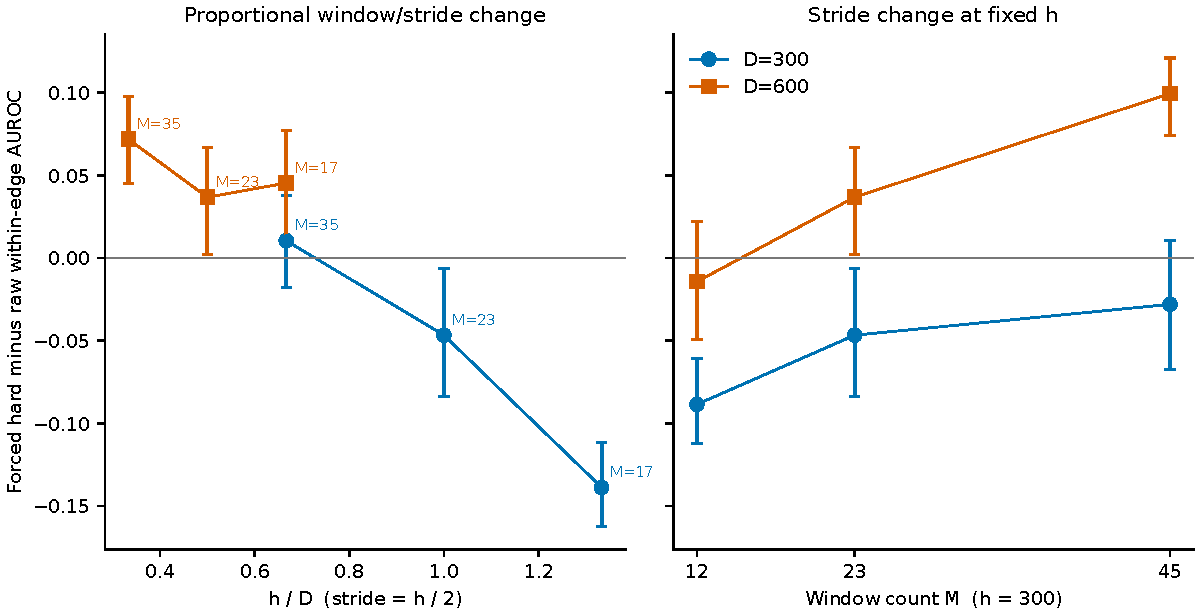
\includegraphics[width=\linewidth]{results/information_sciences/narrative_assets/fig_symmetric.pdf}
\caption{Study C: forced-minus-raw within-edge temporal AUROC in 30 independent
repeats per cell. Left varies window size and stride together; labels show
window count. Right holds size at 300 and varies stride, giving $M=12,23,45$.
Lines connect the tested configurations; intervals are pointwise $95\%$
paired-repeat bootstrap intervals.}
\label{fig:symmetric}
\end{figure}

\subsection{Sensitivity of boundary detection to evaluation conventions}
\label{sec:localisation-results}
Boundary assessments change with zero-score treatment and threshold reference
(Figure~\ref{fig:localisation}). For an eligible edge, standard AP exceeds
positive-change AP by $\pi_{\rm boundary}(1-R_+)$, where $R_+$ is the
fraction of true boundary slots with positive predicted strength.
At $D=600$ in Study B, hard-minus-raw standard-AP differences are
$+0.140$, $+0.154$ and $+0.077$ for fixed, random and irregular schedules,
with pointwise intervals above zero. Positive-change AP gives $+0.068$,
$+0.074$ and $-0.022$, with intervals crossing zero.

Amplitude references are also consequential. In B's fixed schedule, q95 F1
favours raw under the common raw-amplitude threshold, with hard-minus-raw
$-0.077$ $[-0.093,-0.060]$, and favours hard under each method's own
q95, with $+0.223$ $[0.178,0.268]$. In C's $300/150$ grid at $D=600$,
the respective contrasts are $-0.100$ $[-0.122,-0.079]$ and $+0.150$
$[0.093,0.206]$; its standard-AP contrast is $+0.040$ $[-0.020,0.104]$.

These comparisons describe different operating rules for the same predictions.
Method-relative quantiles remove uniform positive rescaling but do not
calibrate equal false-alarm rates, and exact zero ties remain relevant.
Shrinkage preserves both AP definitions and method-relative F1 on these
outputs while potentially lowering common-threshold F1. Supplement Section~S5
reports all five fixed quantiles and stable-edge rates, with no selection of
an optimal F1 on the evaluation truth.

\begin{figure}[!htbp]\centering
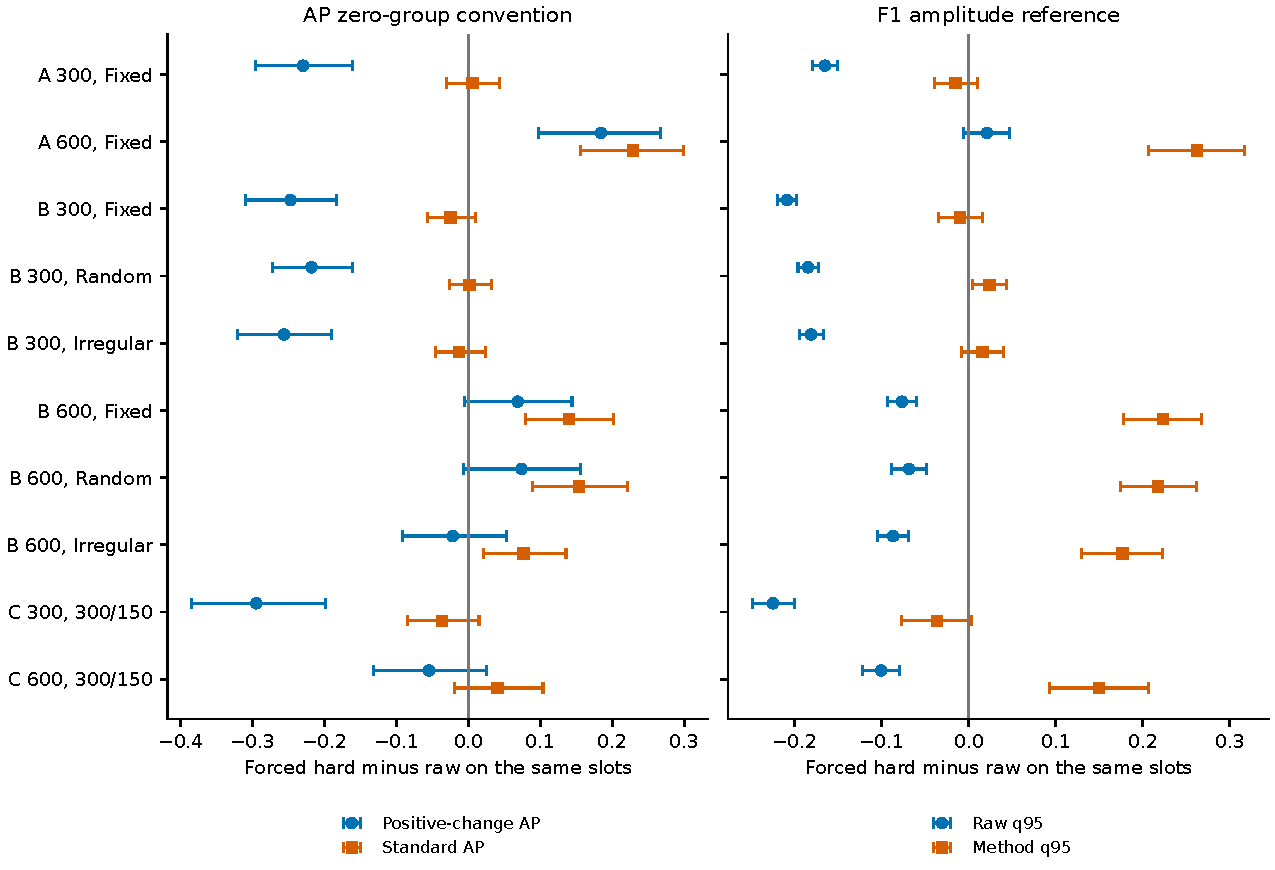
\includegraphics[width=\linewidth]{results/information_sciences/narrative_assets/fig_boundary_sensitivity.pdf}
\caption{Boundary sensitivity on unchanged predictions, hard minus raw.
Left compares positive-change AP with standard AP including the zero-score
group. Right compares a shared raw q95 amplitude threshold with each method's
own q95. All differences use the same cell's slots; C shows the central
$300/150$ setting. Intervals are $95\%$ pointwise paired-repeat bootstrap
intervals using shared within-cell resamples. Full grids, stable edges and
both AP conventions are reported in Supplement Section~S5.}
\label{fig:localisation}
\end{figure}

\subsection{Evaluation beyond recurrent clustering}
\label{sec:external-framework}
A segmentation-and-refit framework exhibits a related separation between
pooled and temporal gains (Table~\ref{tab:external-framework}). On Study C's
30 paired repeats at each duration and the $300/150$ grid, penalised PELT
partitions the raw window features into contiguous segments. A VAR-Lasso
model is then fitted independently on each non-overlapping segment range.
This comparison uses our graph-estimation adapter to the external change-point
algorithm; it estimates segment count and uses neither recurrent K-means
grouping nor the acceptance gate.

Relative to raw windows, PELT plus VAR increases pooled AUROC by $+0.013$
$[0.006,0.020]$ at $D=300$ and $+0.008$ $[0.001,0.014]$ at
$D=600$. Within-edge temporal AUROC differences are $+0.005$
$[-0.020,0.027]$ and $-0.006$ $[-0.020,0.008]$, leaving the temporal
comparison inconclusive at both durations. At $D=600$, positive-change AP
gives $-0.125$ $[-0.205,-0.044]$ while standard AP gives $-0.011$
$[-0.067,0.048]$. Thus both the evaluation target and zero-score convention
affect the comparison outside recurrent clustering.

All 60 cases and 644 segment refits converge. The fixed configuration yields
9--11 segments on 23 windows, reaching the 11-segment minimum-length cap in
45 cases. Supplement Section~S6 provides the settings, counts and paired
results, alongside the distinct auxiliary seven-window segmentation study.

\begin{table}[!htbp]\centering
\caption{A different segmentation/refit structure on Study C's
$300/150$ grid, 30 paired repeats per duration. Within-edge denotes within-edge
temporal AUROC. Standard AP includes the zero-score group. F1 uses raw-shared or
method-specific q95, without selecting a best operating point. Paired
differences use unrounded repeat values and appear in Supplement Section~S6.}
\label{tab:external-framework}
\resizebox{\linewidth}{!}{\begin{tabular}{rlrrrrr}
\toprule
$D$ & Method & Pooled AUROC & Within-edge & AP$_{\rm std}$ & F1$_{\rm raw}$ & F1$_{\rm self}$ \\
\midrule
300 & Raw & 0.765 & 0.707 & 0.665 & 0.268 & 0.268 \\
300 & Forced hard & 0.872 & 0.661 & 0.628 & 0.043 & 0.231 \\
300 & PELT + VAR & 0.779 & 0.712 & 0.834 & 0.321 & 0.333 \\
600 & Raw & 0.786 & 0.761 & 0.440 & 0.230 & 0.230 \\
600 & Forced hard & 0.901 & 0.797 & 0.480 & 0.130 & 0.380 \\
600 & PELT + VAR & 0.794 & 0.754 & 0.429 & 0.222 & 0.238 \\
\bottomrule
\end{tabular}
}
\end{table}

\FloatBarrier

\section{Discussion and conclusions}
\label{sec:discussion}
Aggregation changes two kinds of comparisons: ordering different edges and
ordering the active and inactive windows of one edge. The experiments show
why these effects deserve separate evaluation. Hard aggregation improves
pooled ranking at both duration configurations in Study A, while its
within-edge temporal effect changes sign. Shrinkage achieves pooled gains
without grouping, and residual emission restores comparisons that hard
maps tie. The fixed local scores make these changes attributable to the
emission intervention in the evaluated systems.

The two-state factorisation provides a useful account of relative benefit.
The product of state-assignment discrimination and graph-contrast concordance
must be interpreted against the temporal ranking already present in raw
scores. Better grouping or clearer graph contrast can therefore coexist with
little relative gain when the local scores already discriminate active windows
well. These ground-truth diagnostics explain an observed configuration;
their empirical factors are jointly estimated.

Windowing and execution rules define further conditions of the comparison.
Duration changes at fixed record length alter switch coverage, and Study C
shows substantial variation across window and stride settings under a common
generator. The fixed gate often rejects useful candidates in the longer
records. Static fallback then removes temporal variation altogether, whereas
raw fallback preserves the local ranking on those rejected cases. Reporting
acceptance and the accepted subset's own paired raw comparison makes this
execution effect visible.

For evaluation practice, the results support three complementary reports:
pooled or target-specific structural ranking, within-edge temporal AUROC,
and boundary detection with explicit zero-score and threshold conventions.
Stable-edge changes and gate acceptance complete the operational picture.
The PELT/refit comparison shows the value of this separation for another
partition/refit structure. Reference labels determine which of these reports
are possible: the ESS industrial benchmark supplies a static expert graph,
supporting an external-data alignment illustration in Supplement Section~S7,
while temporal discrimination and boundary recovery require time-indexed truth.

The empirical scope is two-state linear switching systems and local linear
scorers. The clustering experiments use a supplied state count, and the PELT
adapter estimates a segment count from the same local-score features.
Study C's generator modifications are evaluated jointly, so their individual
effects remain unresolved. The auxiliary GMM responsibilities are nearly
binary and provide limited evidence about diffuse soft aggregation.
These conditions identify useful directions for extending the evaluation
protocol to other scorers, state structures and nonlinear systems.

Structural ranking, within-edge temporal discrimination and boundary detection
answer distinct recovery questions. Shared-score controls and diagnostic
accounting make that distinction operational, explaining how an aggregation
rule can improve one answer while weakening another.


\paragraph{Data and code availability.}
Simulation inputs, fitted outputs, analysis code and figure/table generation
tools are included in the accompanying reproducibility archive,
\nolinkurl{information_sciences_reproducibility.zip}. Its README provides separate
routes for recomputing saved results and generating and fitting new runs;
Supplement Section~S8 describes the environment and selected same-seed
reproduction checks.
The source code and complete archive are available in version
\texttt{v2026.10.27} at
\url{https://github.com/xschang1002/latent-state-graph-recovery/releases/tag/v2026.10.27}.

\paragraph{Funding and competing interests.}
This research received no external funding. The author declares no competing
interests.

\paragraph{CRediT authorship contribution statement.}
Xuansong Chang: Conceptualization, Methodology, Software, Validation, Formal
analysis, Investigation, Data curation, Visualization, Writing -- original draft,
Writing -- review and editing.

\paragraph{Declaration of generative AI use.}
OpenAI Codex assisted code implementation, regression tests, experiment
orchestration, figure preparation, manuscript drafting and editorial revision.
Scientific decisions, interpretation and responsibility for the reported work
and its final publication rest with the author.

\bibliographystyle{plainnat}
\bibliography{paper/references}
\end{document}

